\documentclass[11pt]{article}

%------------%
%  Packages  %
%------------%

\usepackage{amsmath}
\usepackage{amssymb}
\usepackage{amsthm}
\usepackage{bm}
\usepackage{changepage}
\usepackage{float}
\usepackage[margin=1.0in]{geometry}
\usepackage{graphicx}
\usepackage{makecell}

%-----------------%
%  Header/Footer  %
%-----------------%

%\setlength\parindent{0pt}
\title{\bf Simulation of Real-Time Workloads on a Multiprocessor in the Presence of Overhead}
\author{Ryan Gibson\\Department of Computer Science\\University of North Carolina at Chapel Hill\\ragibson@cs.unc.edu}
\date{December 3, 2019}

\newcommand{\singlespace}{\baselineskip0.16truein}
\newcommand{\figref}[1]{Figure~\ref{#1}}
\newcommand{\secref}[1]{Section~\ref{#1}}
\newcommand{\tabref}[1]{Table~\ref{#1}}

\begin{document}
	\maketitle
	
	\begin{abstract}
		We present a simulation environment that evaluates the schedulability of task sets by explicitly generating schedules until a deadline is missed. We support several global multiprocessor scheduling algorithms and a simple model of overhead accounting that includes context switch costs and cache warming behavior. We use this to perform a simulation study and determine the rough effects of cache on multiple scheduling algorithms.
	\end{abstract}

\section{Introduction}
\label{sec:Introduction}

Real-time scheduling algorithms have seen widespread use across a range of applications and industries in which tasks are associated with hard timing constraints. In such cases, deadline misses may have particularly catastrophic effects and must be avoided (if possible). For instance, a signal processing application may permanently lose data from a sensor if it is not processed by the next sensor update, an aircraft may become inoperable if critical flight control routines run too infrequently, and a self-driving car may crash into nearby vehicles or pedestrians if obstacle-avoidance routines fail to detect collisions with sufficient warning.

However, despite its extensive application in safety-critical systems, most of the fundamental results from the real-time literature focus on ideal systems in which processors run with zero overhead. The inclusion of context switch costs and the behavior of modern CPU caches significantly complicates the theoretical approaches required to prove that a particular scheduling scheme will prevent deadline misses. As such, these overheads are frequently ignored in real-time scheduling analysis. Indeed, proper overhead accounting in real-time systems remains an active area of research.

In developing a simulation environment that supports a restricted model of processor overheads, we hope that we can construct more realistic ``rules of thumb'' as to how specific real-time workloads should be scheduled. These could be used to guide the design and implementation of future real-time systems, even when formal guarantees of timeliness in the presence of processor overhead are beyond the theoretical abilities of the research community at large.

The rest of this paper first briefly discusses related work in
\secref{sec:RelatedWork} and then describes our simulation environment in
\secref{sec:SimulationEnvironment}. \secref{sec:SimulationStudy} presents the construction of our simulation study on a fixed task set distribution and its results are given in \secref{sec:Results}. \secref{sec:Conclusion} discusses our
conclusions and describes potential future work.

\section{Related Work}
\label{sec:RelatedWork}

Other real-time scheduling simulators have been developed, with particular emphasis on their use as a teaching tool.

In \cite{Diaz}, Diaz et al.\ released ``Realtss'' to serve as a research and teaching tool in order to promote the ongoing development of existing Real-Time Operating Systems (noting that, at the time, ``almost every existing real-time operating system [provided] only POSIX-compliant fixed priority scheduling''). However, their approach focused only on ideal uniprocessors and restricted analysis to a few metrics including utilization, response time, and the number of observed deadline misses.

Another teaching tool, ``RTSim'' was presented by Manacero et al.\ in \cite{Manacero}. As opposed to Realtss, this tool expanded focus into multiprocessor scenarios. It has been used in education to simulate task set execution in order to demonstrate the implications of various scheduling algorithms and policies.

A particularly notable simulator, ``Cheddar'', was developed by Singhoff et al.\ \cite{Singhoff}. As of June 2019, this tool is still under active development and allows for the analysis of a wide range of uniprocessor and multiprocessor scheduling policies. It also allows for comparing schedules based on number of context switches as well as cache-related preemption delays.

We in no way propose that our tool is ``better'' than these alternatives (indeed, our tool completely omits resource control, for example), but hope that its simplicity lends itself towards potential future use. Moreover, our tool is one of the first that attempts to directly model cache behavior and the associated increase in execution rate over time.

\section{The Simulation Environment} % TODO: Rename? Used to be Implementation
\label{sec:SimulationEnvironment} 

Our simulator is written in Python and supports reading/writing task systems from human-readable files. As such, we anticipate that it should be relatively easy to extend and implement in pre-existing workflows by simply redirecting task system generation output into text files. We now discuss the features of our simulator in detail. 

\subsection{Task Model and Random Task Set Generation}

Our simulator operates under the discrete time model and works primarily with periodic tasks $\tau_i = (\phi_i, T_i, C_i, D_i)$. As is standard, these tasks release jobs starting at $\phi_i$ and every $T_i$ time units afterwards. Each job has execution cost $C_i$ and must complete by $D_i$ time units after its release.

In our simulator, a task $\tau_i$ with period $T_i = \infty$ operates as a one-shot job -- this task will release a single job with release time $\phi_i$ and deadline $\phi_i + D_i$.

We support generating random task sets by drawing uniformly from four user-defined sets of values, $R_\phi$, $R_T$, $R_C$, and $R_D$ corresponding to the possible values for the task phases, periods, execution costs, and relative deadlines, respectively.

As previously mentioned, we also support completely user-defined task sets as input from text files, so custom task generation procedures can be added with ease.

\subsection{Scheduling Algorithms}

For uniprocessor scheduling, we support Rate-Monotonic, Deadline-Monotonic, Static-Priority (user-defined priorities), Earliest-Deadline-First, and Least-Laxity-First scheduling as well as the non-preemptive versions of these policies.

For multiprocessor scheduling, we support the global scheduling policies arising from these (preemptive and non-preemptive) uniprocessor scheduling algorithms in both the restricted migration (where tasks can only migrate between jobs) and full migration variants. We also support the PD$^2$ scheduling algorithm from \cite{Srinivasan}.\footnote{For jobs with arbitrary deadlines, we choose to set task weights by $wt(T) = \max\left(\frac{C_i}{T_i}, \frac{C_i}{D_i}\right)$. With this convention, we found it necessary to add a third tie-break in the priority definition for PD$^2$.

We say that a job ``must execute immediately'' at time $t$ if its remaining execution cost is equal to the remaining time until its deadline. In the case of a subtask deadline tie, we favor jobs that must execute immediately, regardless of successor bits and group deadlines.

This new tie-break is necessary when tasks have relative deadlines less than periods since the system can have total weight exceeding $m$ (the number of processors). In this case, it can be mandatory to schedule a job with zero successor-bit when the standard PD$^2$ tie-breaks would choose otherwise. A simple example of this is a task with $C_i=D_i$ -- such a task has weight 1 and windows that do not overlap, so it would lose all tie-breaks involving a successor bit \Big($b(T_i) = \left\lceil\frac{i}{wt(T)}\right\rceil - \left\lfloor\frac{i}{wt(T)}\right\rfloor = i-i =0$ in this case\Big), but must be scheduled whenever eligible or else it will miss its deadline.

Indeed, the task system in \figref{fig:Pfair_multiprocessor_plot} will miss deadlines under PD$^2$ scheduling with our task weight convention if this third tie-break is omitted.}

In this paper, we will always break priority ties in these algorithms in favor of currently executing jobs.

Unless otherwise specified, our simulator explicitly generates schedules until a deadline is missed or until we are guaranteed that no deadlines will ever be missed. In the case of synchronous periodic task systems (when all phases are zero), we are guaranteed that a deadline miss must occur by the hyperperiod of the task system (at which point the sequence of job releases repeats), so by default we only construct schedules up to this point.

In the asynchronous case, we guarantee that no deadline misses will occur by using a result from Leung and Merill in \cite{Leung} and its generalization by Baruah et al.\ in \cite{Baruah}. This gives that an infeasible task system $\bm{\tau}=\{\tau_1, \dots, \tau_n\}$ with utilization $\sum_{i=1}^n \frac{C_i}{T_i} \leq 1$ will miss a deadline on a uniprocessor by time $2 \cdot H + \max_{1 \leq i \leq n}\{\phi_i\} + \max_{1 \leq i \leq n}\{D_i\}$ where $H$ is the hyperperiod of $\bm{\tau}$. Similarly on a multiprocessor, the sequence of job releases of $\bm{\tau}$ will repeat by time $2 \cdot H + \max_{1 \leq i \leq n}\{\phi_i\}$ and all jobs released by this time will have deadlines at or before $2 \cdot H + \max_{1 \leq i \leq n}\{\phi_i\} + \max_{1 \leq i \leq n}\{D_i\}$. Hence in this case, our simulator defaults to only constructing schedules up to this point in time.

\subsection{Overhead Model}

Our simulator allows five overhead parameters to be specified on a per-processor basis: the cost $s$ to schedule a job, the cost $d$ to dispatch a job, the cost $p$ to preempt/resume a job, the cache warmup time $t_\text{warmup}$, and the final (``warm cache'') execution rate $r_\text{max}$.

The first three overhead parameters $s,d,p$ induce additional \emph{nonpreemptive} execution cost\footnote{The nonpreemptive execution of overhead here is necessary to prevent, for example, job preemptions that would occur in the middle of a context switch. On a real system, such preemptions are clearly impossible.} (which we will refer to as ``overhead'') that jobs take on as follows.

\begin{itemize}\itemsep0em
	\item When a job is first scheduled, its execution cost is inflated by $s+d$ time units of overhead for the initial scheduling and dispatch.
	\item When a job is resumed, its execution cost is inflated by $d+p$ time units of overhead if the processor of interest was previously idle and is otherwise inflated by $d+2p$ time units of overhead. This accounts for the context switches induced by both the preempted and the preempting jobs.
\end{itemize}

The last two overhead parameters $t_\text{warmup}$ and $r_\text{max}$ allow for a simple model of the initial slowdown caused by processors that run with very little of their data in cache. This affects job execution in the following ways.

\begin{itemize}\itemsep0em
	\item Each processor has an associated execution rate that determines how much a scheduled job's remaining execution cost decreases with each time unit. When a job is scheduled, this starts at 1 and increases linearly to $r_\text{max}$ after $t_\text{warmup}$ units of consecutive execution.
	\item Importantly, job overhead always runs with an execution rate of 1 and this execution does \emph{not} increase the execution rate of a processor.\footnote{In analogy to a real system, processes do not fill cache lines in any useful manner \emph{during} a context switch or when dispatching jobs.}
	\item Job completion times are rounded up to the next integral time unit when necessary to maintain the discrete time model used by our simulator.
\end{itemize}

\subsection{Sample Graphical Output}

Our simulator includes three plotting methods, one intended for use with uniprocessor schedules and two for multiprocessor schedules. We describe these below and present some simple examples of their output.

\subsubsection{Uniprocessor Schedules}

For uniprocessor schedules, our simulator plots show one task per row with job releases marked by blue, upward pointing arrows and job deadlines marked by red, downward pointing arrows. The intervals of time in which jobs are scheduled are shown as filled rectangles and job completions are denoted with a ``T'' shape. We show an example schedule with this plot style in \figref{fig:RM_uniprocessor_plot}.

\begin{figure}
	\centering
	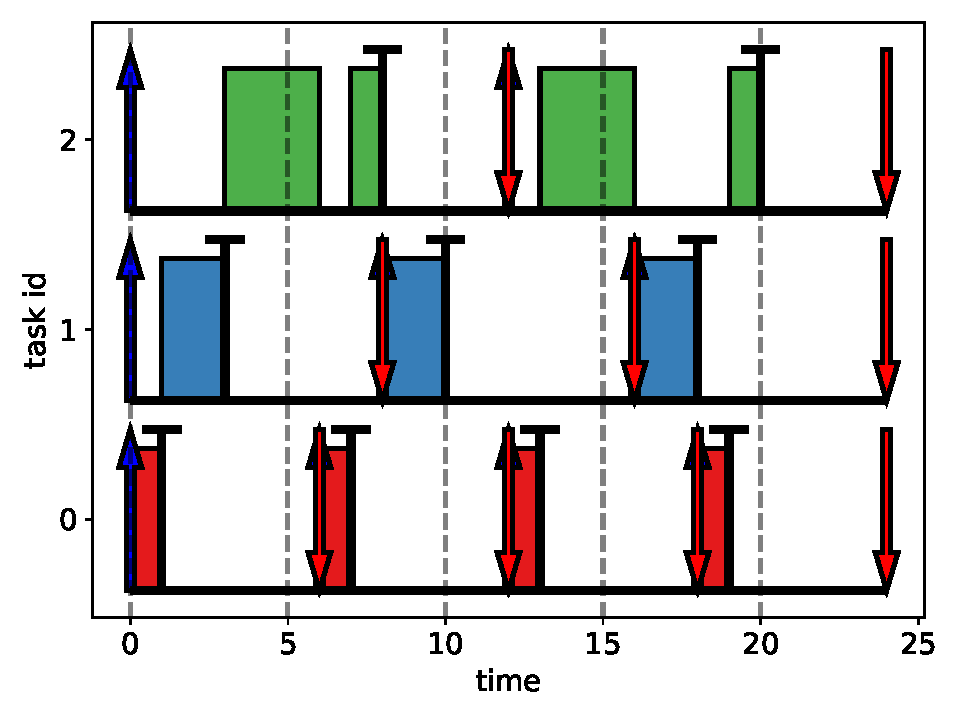
\includegraphics[width=8cm]{RM_uniprocessor_example.pdf}
	\caption{An example uniprocessor schedule using the Rate-Monotonic algorithm. The task system shown here is $\tau_0=(6,1)$, $\tau_1=(8,2)$, $\tau_2=(12,4)$ on the time interval $[0, 24]$.}
	\label{fig:RM_uniprocessor_plot}
\end{figure}

\subsubsection{Multiprocessor Schedules}

For multiprocessor schedules, our simulator has two styles of plots, one that plots one task per row and one that plots a processor in each row.

The style with one task per row uses the same notation as with uniprocessor schedules, but colors tasks based on which processor they are scheduled on. By contrast, the plots with one processor per row are colored based on which task is scheduled in each interval. We show two example schedules with both plot styles in \figref{fig:EDF_multiprocessor_plot} and \figref{fig:Pfair_multiprocessor_plot}.

\begin{figure}
	\centering
	\phantom{spacing}
	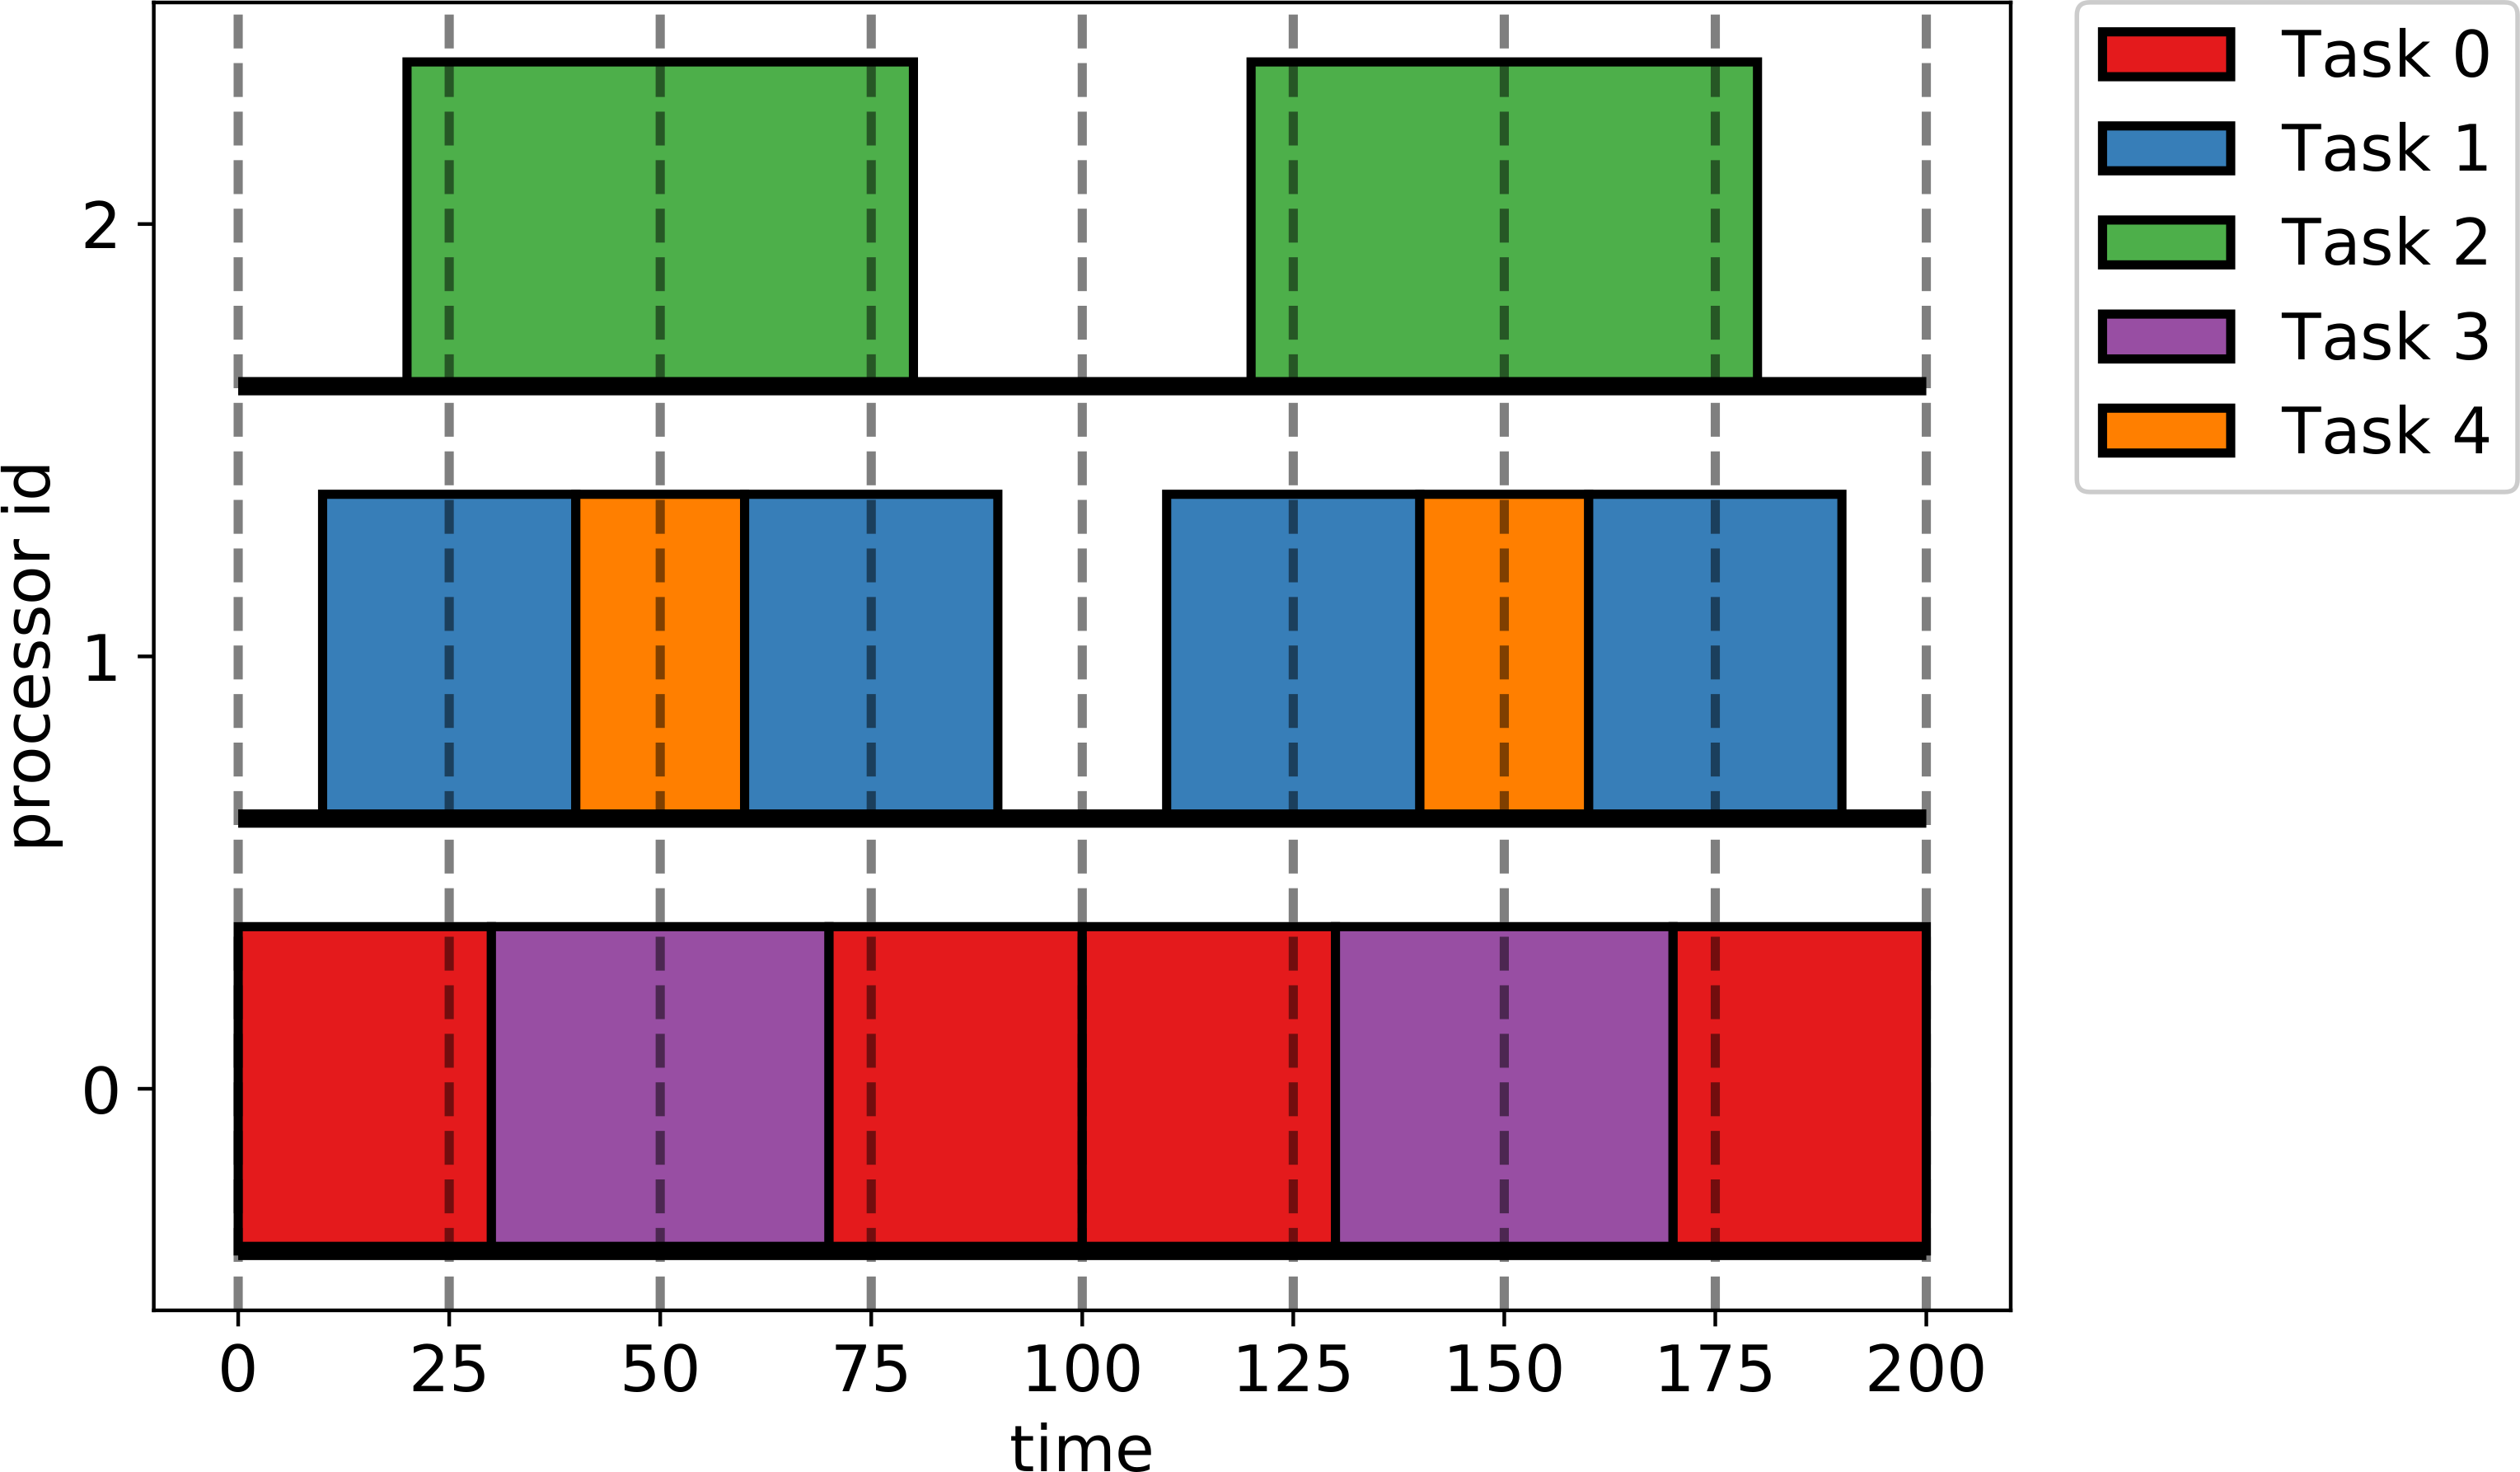
\includegraphics[height=4.55cm]{EDF_multiprocessor_example1_combined.png}\quad
	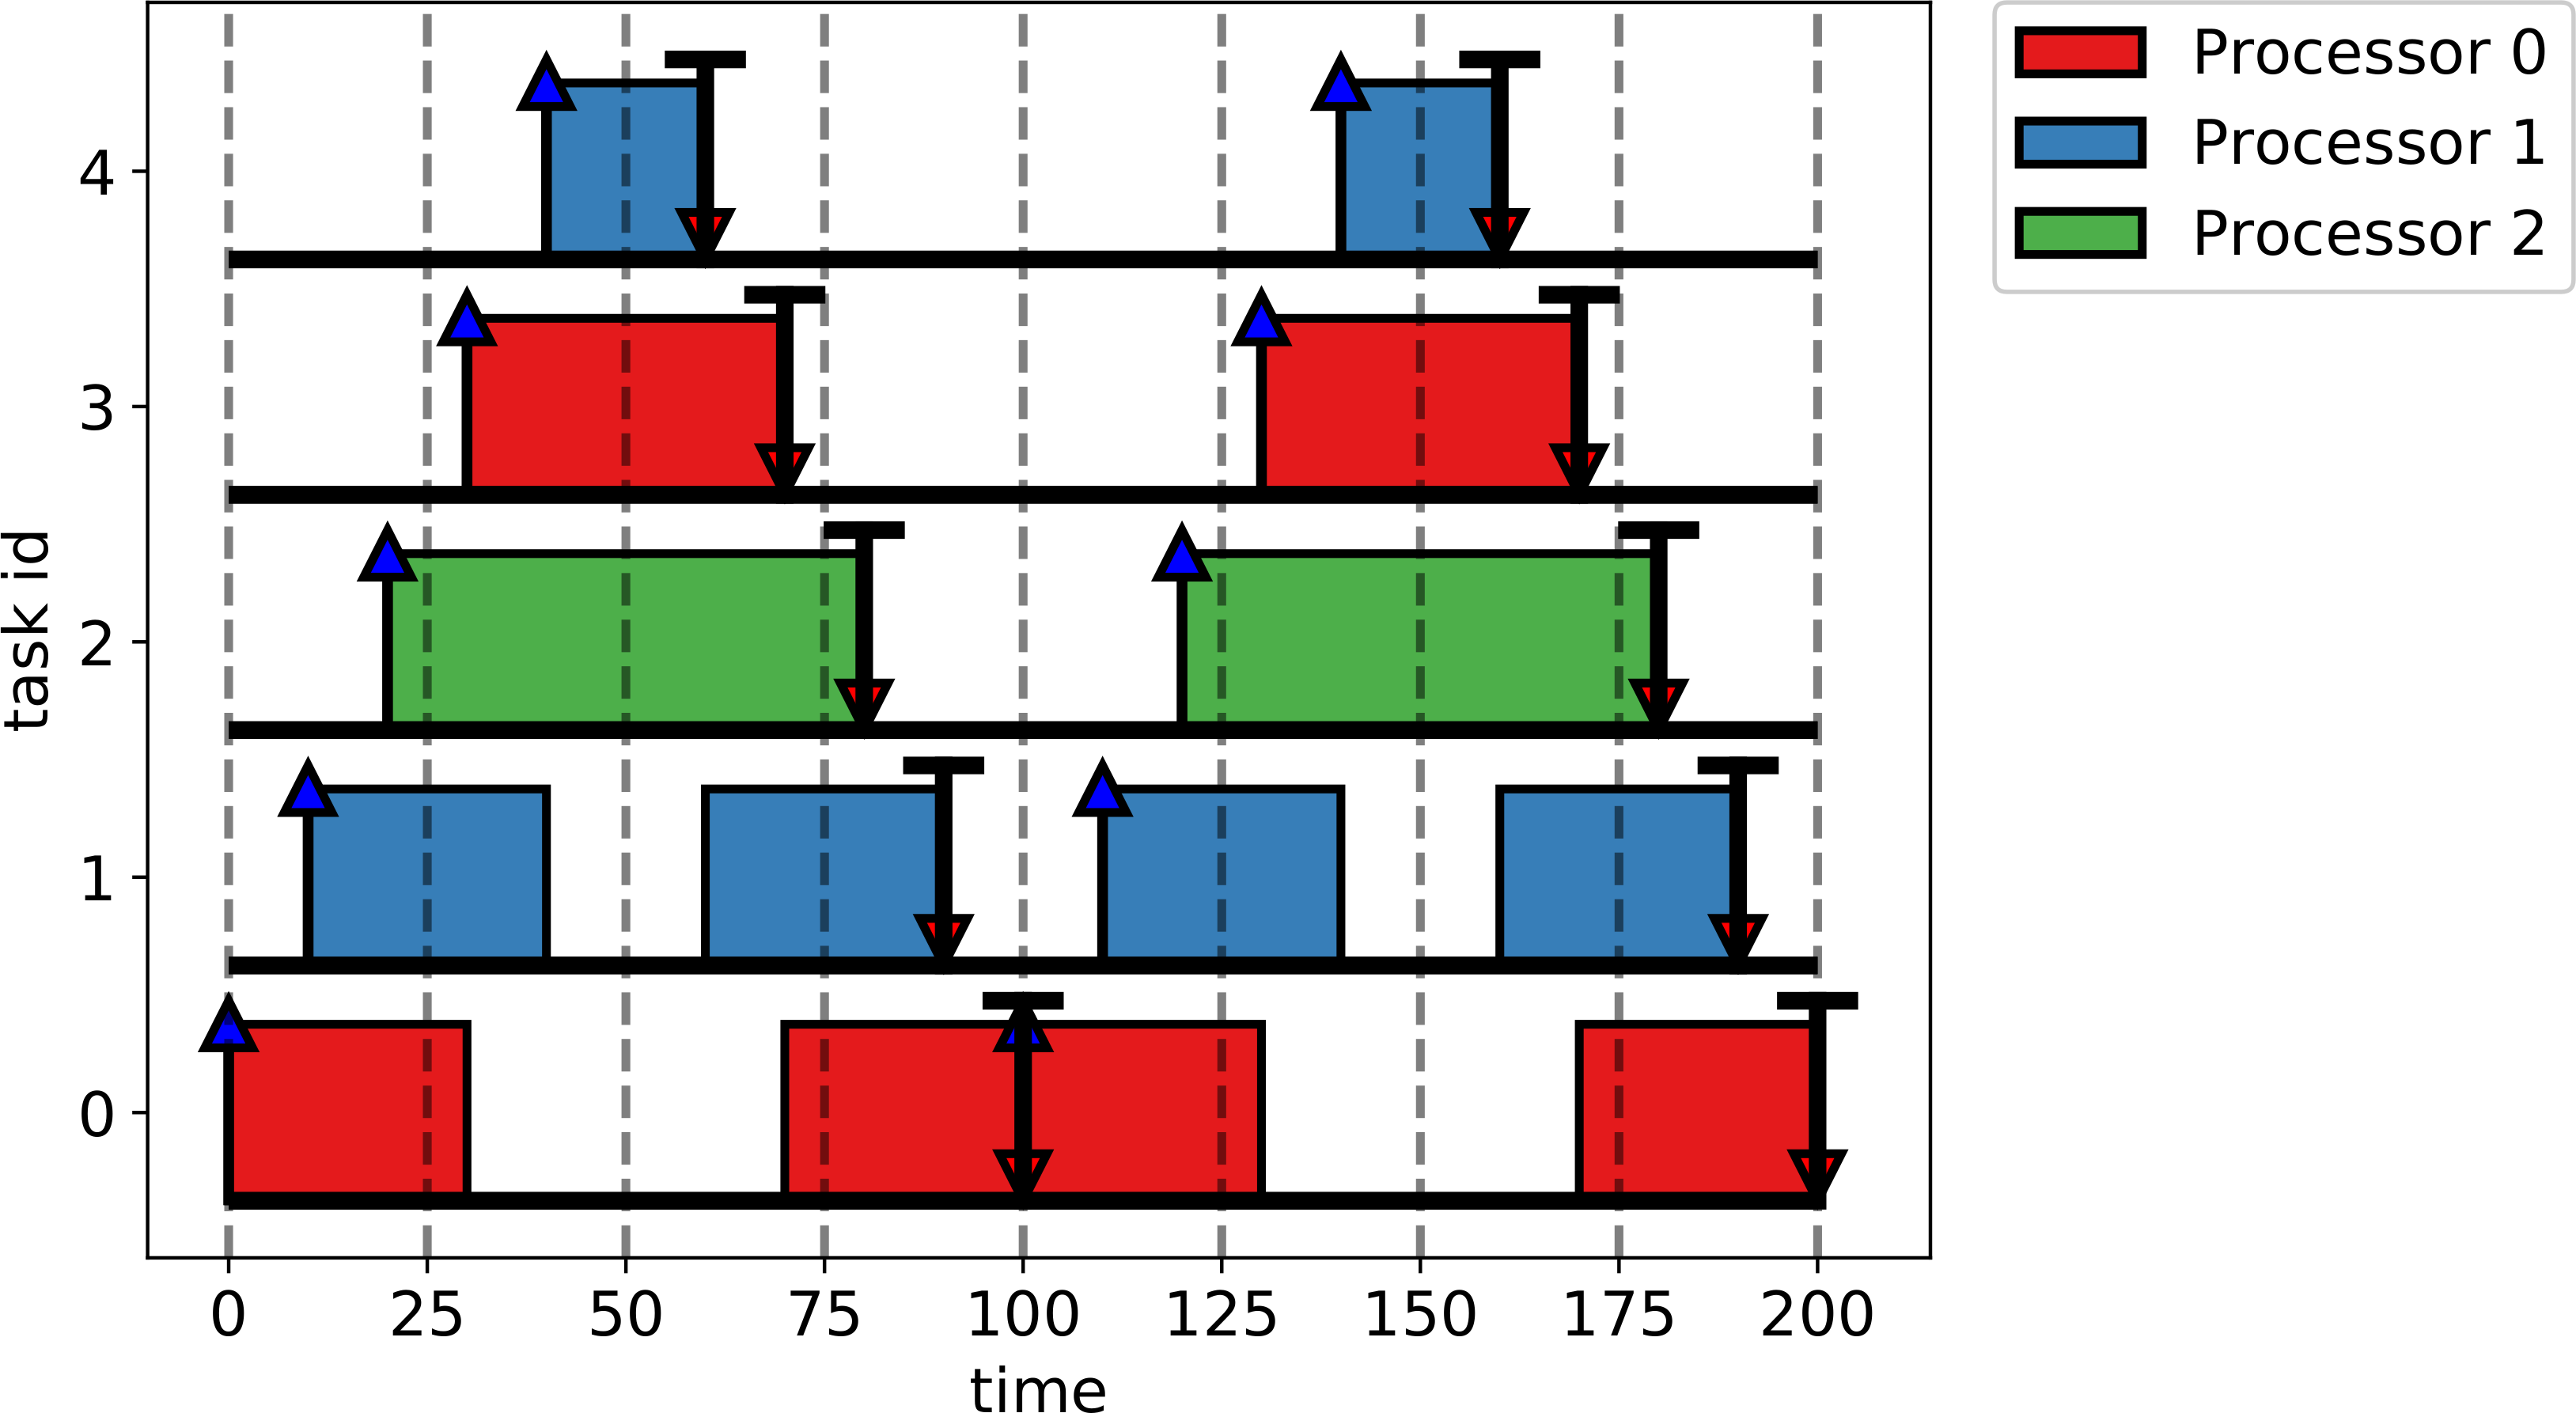
\includegraphics[height=4.55cm]{EDF_multiprocessor_example2_combined.png}
	\caption{An example multiprocessor schedule using the Global Earliest-Deadline-First algorithm on 3 processors. The task system shown here is $\tau_0 = (0,100,60,100)$, $\tau_1 = (10,100,60,80)$, $\tau_2=(20,100,60,60)$, $\tau_3=(30,100,40,40)$, $\tau_4=(40,100,20,20)$ on the time interval $[0, 200]$.}
	\label{fig:EDF_multiprocessor_plot}
\end{figure}

\begin{figure}
	\centering
	\phantom{spacing}
	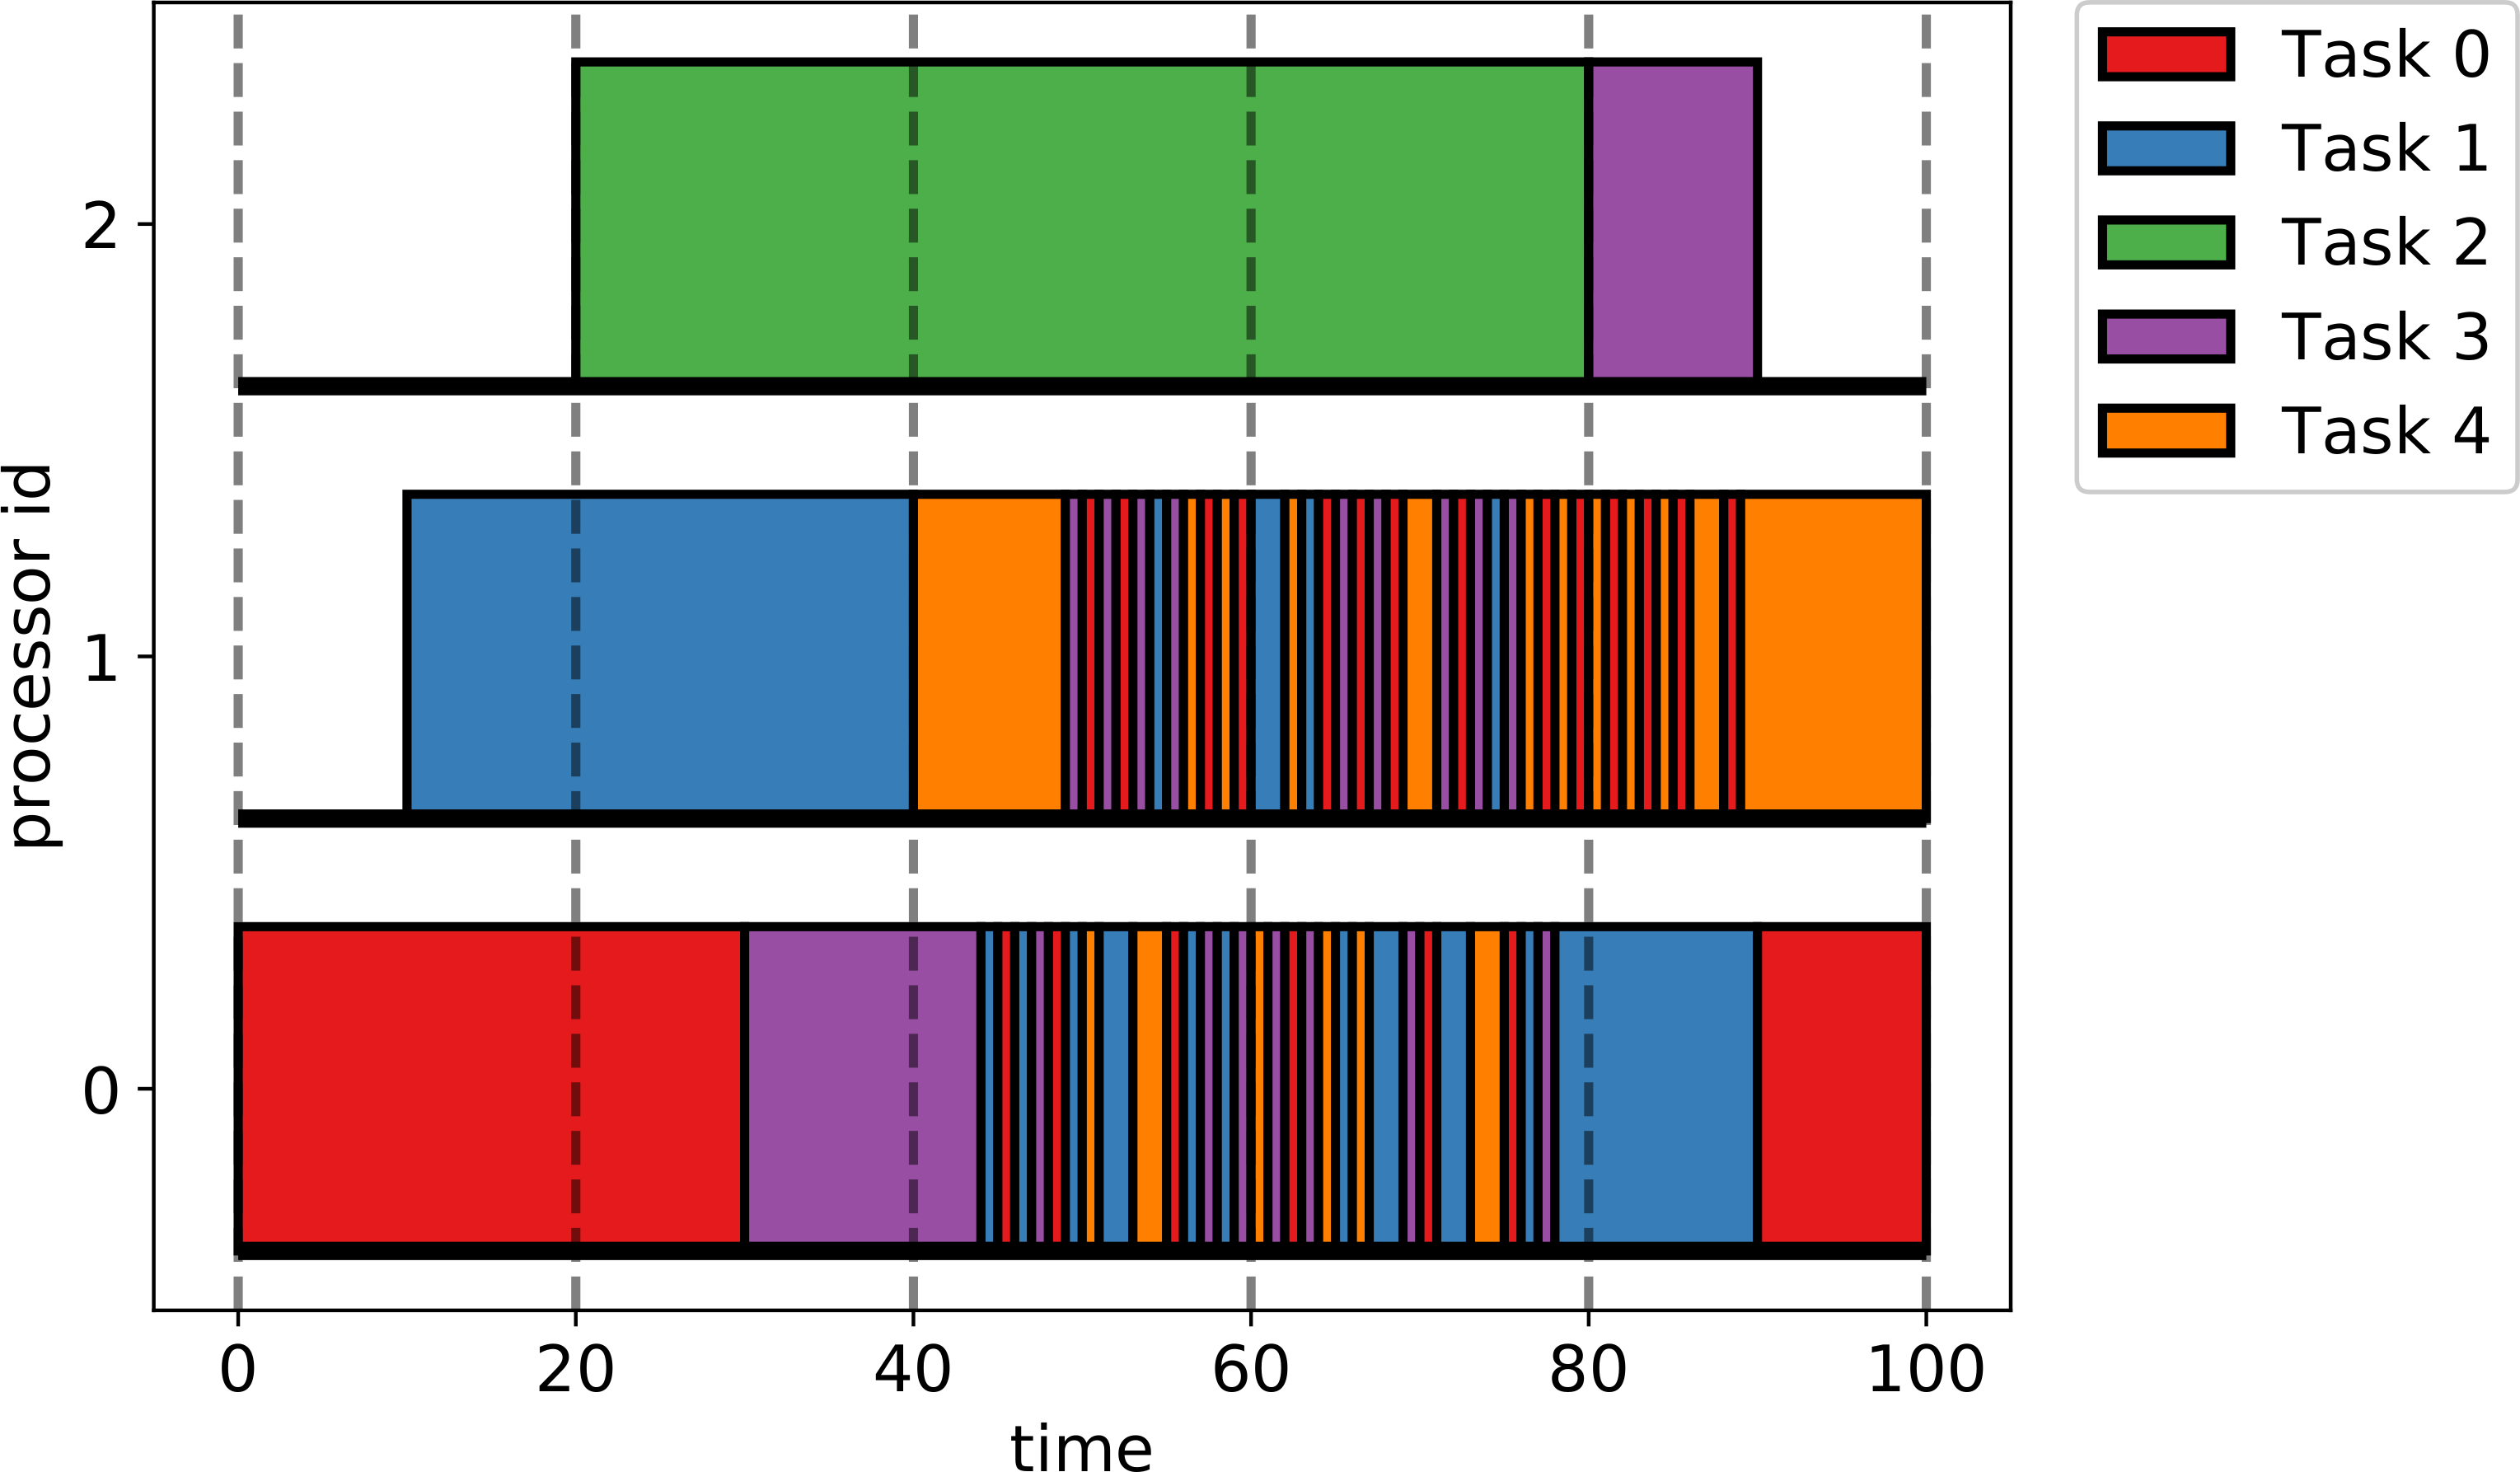
\includegraphics[height=4.55cm]{Pfair_multiprocessor_example1_combined.png}\quad
	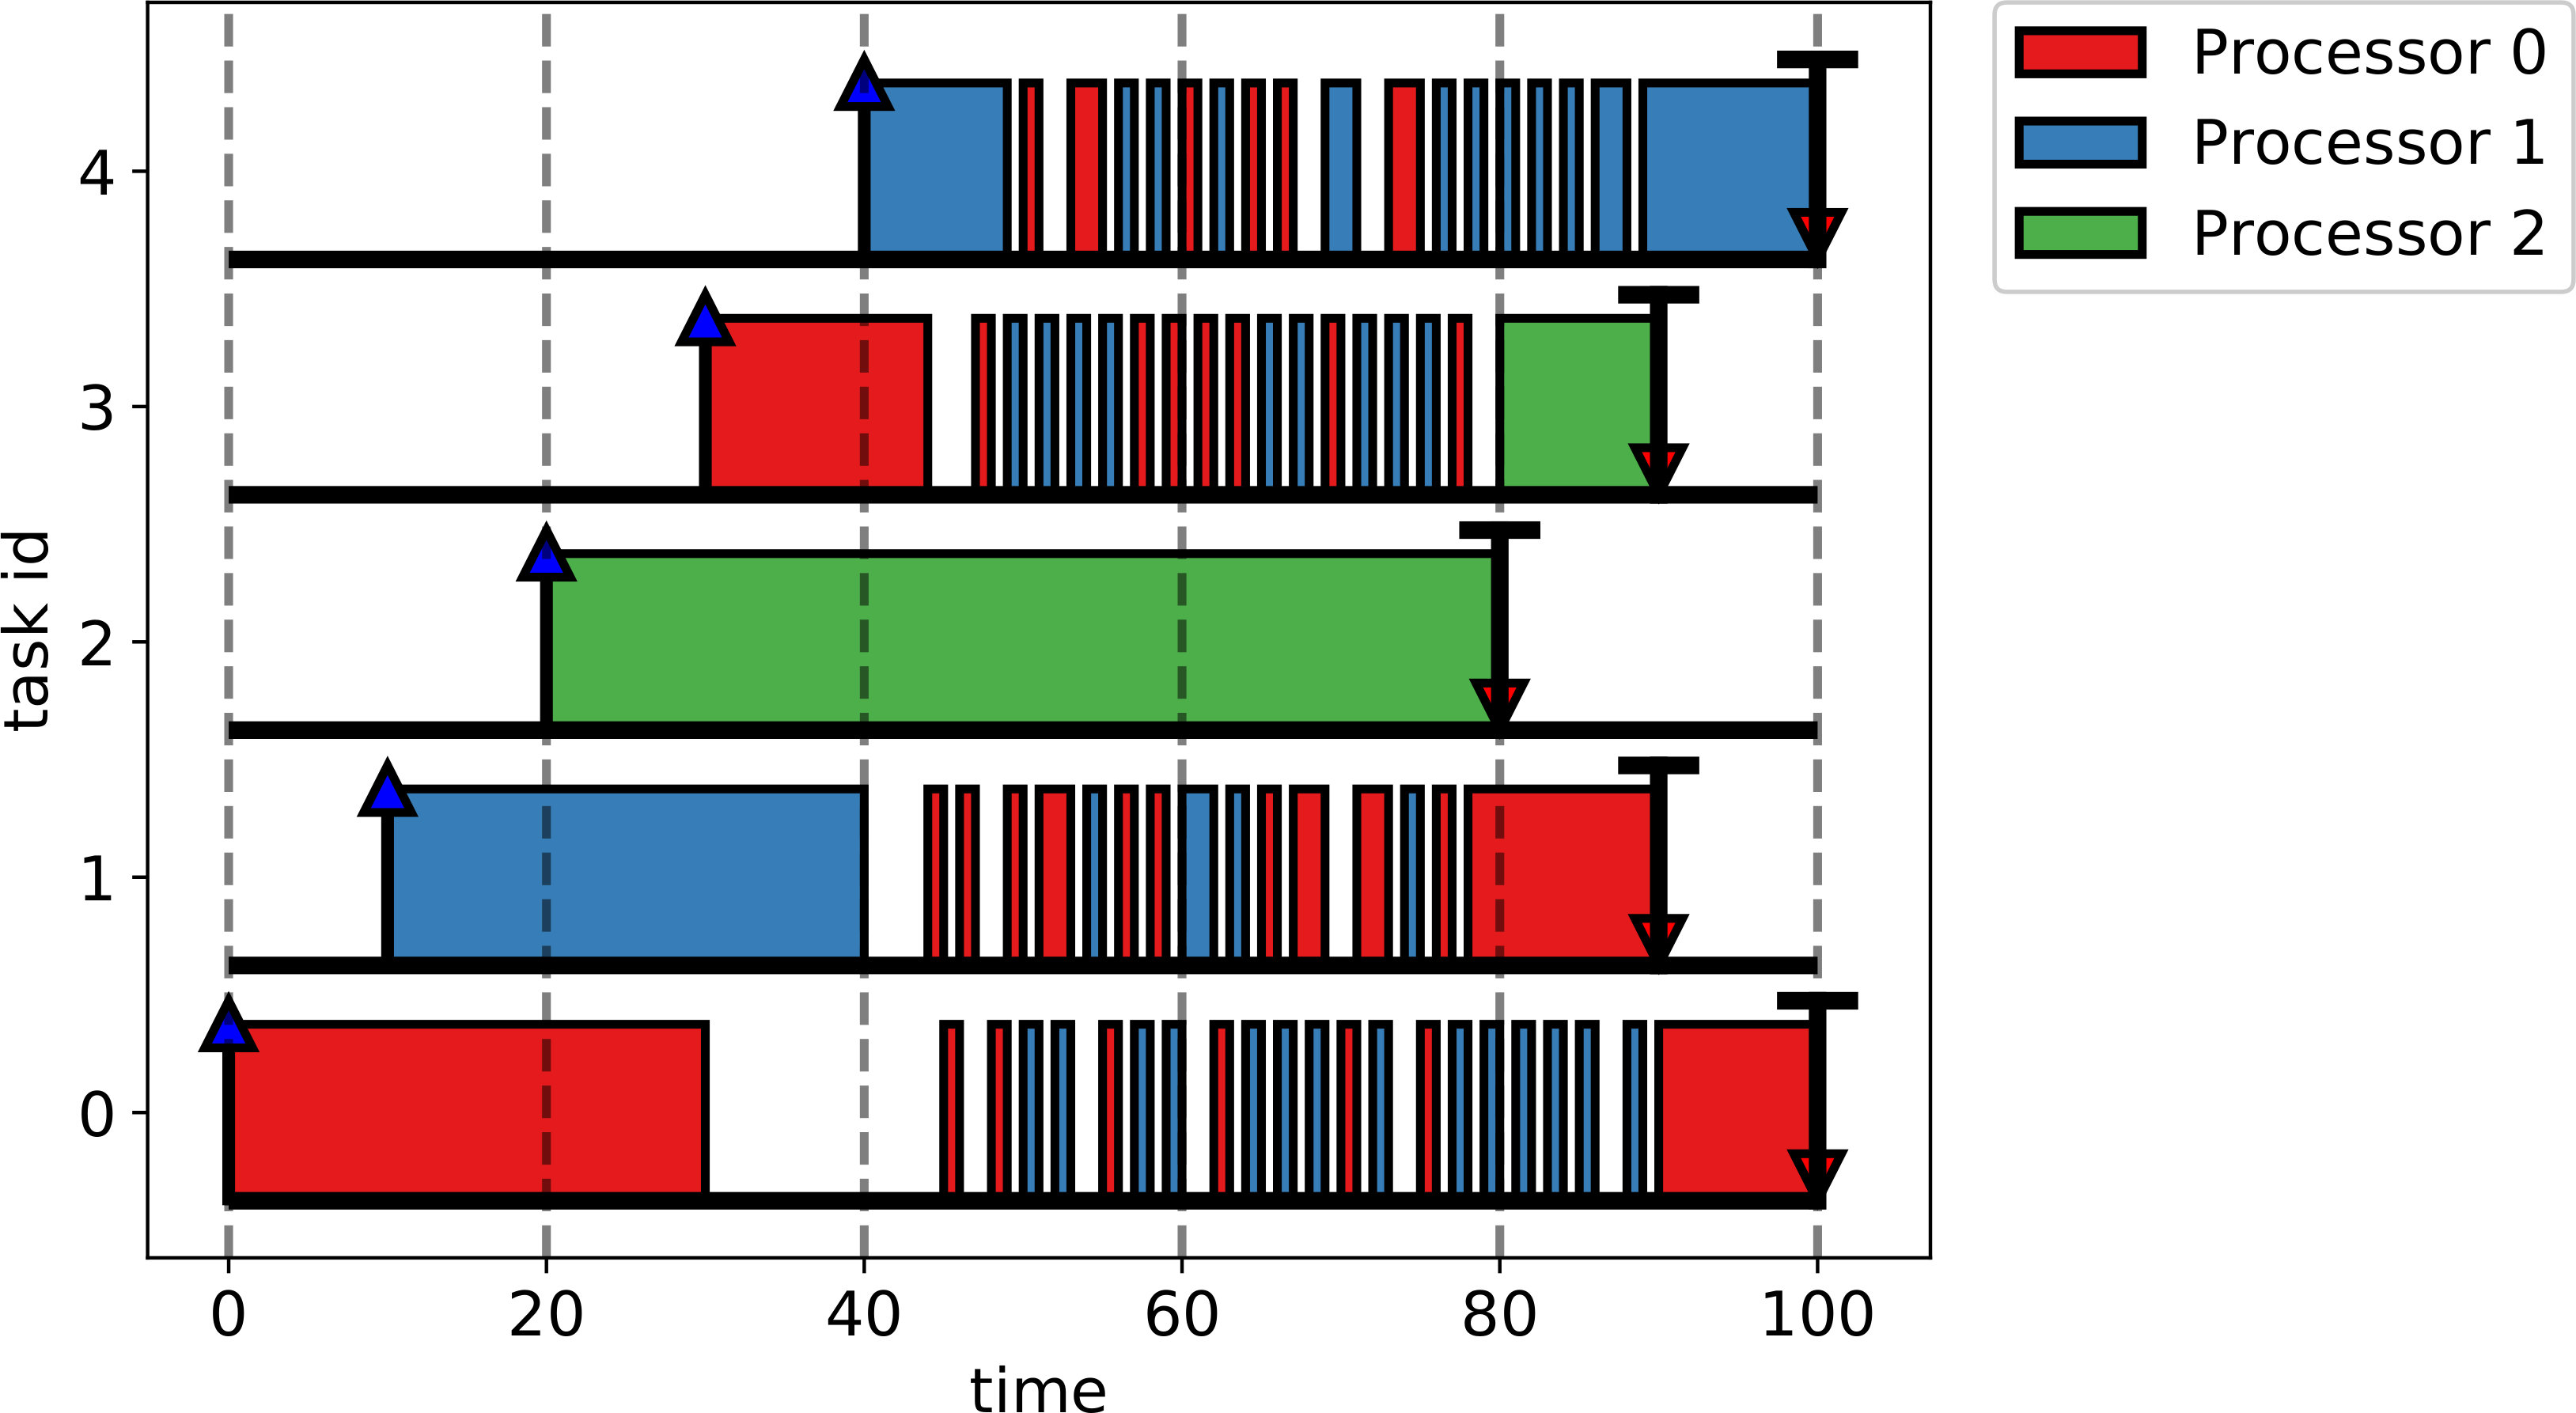
\includegraphics[height=4.55cm]{Pfair_multiprocessor_example2_combined.png}
	\caption{An example multiprocessor schedule using the PD$^2$ algorithm on 3 processors. The task system shown here is $\tau_0 = (0,100,60,100)$, $\tau_1 = (10,100,60,80)$, $\tau_2=(20,100,60,60)$, $\tau_3=(30,100,40,60)$, $\tau_4=(40,100,40,60)$ on the time interval $[0, 100]$.}
	\label{fig:Pfair_multiprocessor_plot}
\end{figure}

\section{The Simulation Study}
\label{sec:SimulationStudy}

Our simulation study evaluates scheduling algorithms by comparing their breakdown densities on randomly generated task sets.

\subsection{Breakdown Density}\label{sec:BreakdownDensity}

For a scheduling algorithm $S$ and task set $\bm{\tau} = \{\tau_1, \dots, \tau_n\}$, we define breakdown density as follows. Consider the reweighted task set $\bm{\tau}'_w = \{\tau_1', \dots, \tau_n'\}$ obtained by inflating/deflating all execution costs by a factor of $w$. That is, $\bm{\tau}'_w$ is the task system composed of tasks $\tau_i' = (\phi_i, T_i, \left\lfloor w*C_i \right\rfloor, D_i)$.

Then, we can find the greatest scaling factor $w$ for which $\bm{\tau}'_w$ is still schedulable under $S$. The resulting density of this task set, $\sum_{i=1}^n \frac{\left\lfloor w \cdot C_i \right\rfloor }{D_i}$ is the breakdown density for $\bm{\tau}$ under $S$. Informally, this gives the largest density that $S$ can schedule for task sets that ``look like'' $\bm{\tau}$.

In this way, higher (average) breakdown densities indicate better scheduling performance as this implies the scheduling algorithm is able to more fully utilize the processor before a deadline miss occurs.

\subsection{Random Task Distribution}\label{sec:TaskDistribution}

Here, we take our discrete time unit to represent 1 $\mu$s and construct random task sets $\bm{\tau} = \{\tau_1, \dots, \tau_n\}$ where each task $\tau_i$ has random period $T_i$ uniformly chosen from \{8000, 16000, 32000, 64000, 128000, 256000\}. Then, we uniformly randomly choose phases $0 \leq \phi_i \leq T_i - 1$, execution costs $1 \leq C_i \leq T_i$, and relative deadlines $C_i \leq D_i \leq T_i$.

Roughly speaking, our intent here to represent a system in which processes must run at approximate frequencies ranging from 4 Hz to 125 Hz (periods ranging from 8 ms to 256 ms). This choice of distribution is somewhat arbitrary, but will demonstrate how our tool can be used to determine rough ``rules of thumb'' as to which scheduling policies are preferable when a task set distribution is known or can be approximated.

\subsection{Choosing Values for the Overhead Parameters}\label{sec:OverheadParameters}

It remains to determine ``realistic'' values for our overhead parameters. Ignoring the effects of cache, modern processors are able to context switch between processes in under 5 microseconds, on average \cite{Li, McVoy}. Hence, since our simulated context switches involve two instances of adding $p$ overhead, we take $p=2$ $\mu$s to be the average cost of preempting/resuming a job in our experiments. Similarly, we take $d=1$ $\mu$s to be our average cost of actually dispatching a job.

The cost $s$ to schedule a job will scale with the complexity of the scheduling algorithm, in general. However, LITMUS\textsuperscript{RT} (a real-time extension of the Linux kernel) is able to maintain scheduling latencies under 4 $\mu$s when using Earliest-Deadline-First plugins on a system with no background processes \cite{Cerqueira}, so we take $s=4$ to be the average cost of scheduling a job in our experiments. We expect that the influence of this particular overhead parameter will be insignificant in comparison to the variable execution rate from our cache model.\footnote{Just as in real systems, the ``indirect'' costs (e.g.\ cache line evictions) of a context switch greatly exceed the ``direct'' costs of simply running the context switch and dispatch code.}

Computing typical values for our cache parameters $t_\text{warmup}$ and $r_\text{max}$ is more complicated since modern CPUs contain a hierarchy of caches of different sizes and speeds. Roughly speaking, these are typically

\begin{itemize}\itemsep0em
	\item L1 caches of size ${\sim}$32KB to ${\sim}$64KB and access times of ${\sim}$1-2 ns
	\item L2 caches of size ${\sim}$256KB to ${\sim}$512KB and access times of ${\sim}$3-6 ns
	\item L3 caches of sizes from ${\sim}$2MB to ${\sim}$20MB and access times of ${\sim}$10-20 ns
	\item For reference, main memory access times are ${\sim}$60-100 ns
\end{itemize}

The access times above are Intel's rough approximations\footnote{Unsurprisingly, these depend on the exact processor architecture and memory being used.} provided in \cite{Levinthal} and the common cache sizes were obtained by surveying Intel's recent CPU architectures in \cite{Intel}.

With 64-byte cache lines filled at the speed of main memory into a completely empty cache, this implies that we have

\begin{itemize}\itemsep0em
	\item L1 cache running at ${\sim}$50x the speed of main memory with $30 \text{ $\mu$s} \lessapprox t_\text{warmup} \lessapprox 100 \text{ $\mu$s}$
	\item L2 cache running at ${\sim}$15x the speed of main memory with $240 \text{ $\mu$s} \lessapprox t_\text{warmup} \lessapprox 800 \text{ $\mu$s}$
	\item L3 cache running at ${\sim}$5x the speed of main memory with $2 \text{ ms} \lessapprox t_\text{warmup} \lessapprox 30 \text{ ms}$
\end{itemize}

In practice, the exact speedup achieved from cache hits depends heavily on the memory access patterns of a particular program. Nevertheless, we will use these approximations to guide our experiments.

\section{Results}\label{sec:Results}

\subsection{Effect of Cache on Uniprocessor Breakdown Density}\label{sec:uniprocessor_breakdown_density_experiments}

We will consider task systems that ``effectively'' utilize the memory hierarchy above the L1, L2, and L3 caches. As such, we generate 25 task systems of 10 tasks each as specified in \secref{sec:TaskDistribution} and evaluate the breakdown densities of several scheduling algorithms under the following overhead schemes.

\begin{itemize}\itemsep0em
	\item ``No cache'' baseline (i.e.\ essentially zero locality of reference): $t_\text{warmup} = 0$, $r_\text{max} = 1$
	\item ``L3 cache'': $t_\text{warmup} = 16000$ $\mu$s, $r_\text{max} = 5$
	\item ``L2 cache'': $t_\text{warmup} = 520$ $\mu$s, $r_\text{max} = 15$
	\item ``L1 cache'': $t_\text{warmup} = 65$ $\mu$s, $r_\text{max} = 50$
\end{itemize}

For instance, the ``L3 cache'' overhead scheme is meant to mimic a system in which all tasks have memory footprints that are too large to fit in the smaller caches (and so the tasks essentially only make effective use of the memory hierarchy above the L3 cache).

Here, we have obtained $t_\text{warmup}$ values by taking the midpoint of the ranges determined in \secref{sec:OverheadParameters} for the L1, L2, and L3 caches. The resulting breakdown densities from our experiments are shown in \tabref{table:uniprocessor_L1_L2_L3_experiment}.

\begin{table}[H]
	\centering
	\resizebox{\textwidth}{!}{%
	\begin{tabular}{|c|c|c|c|c||c|c|c|c|}
		\hline Scheme & EDF & LLF & RM & DM & NP-EDF & NP-LLF & NP-RM & NP-DM\\\hline
		No cache&1.2894&1.1258&1.2476&1.2559&0.5074&0.5071&0.4782&0.4879\\
		L3 cache&1.8343&1.3067&1.7057&1.6911&0.9521&0.9420&0.9011&0.9245\\
		L2 cache&16.8433&3.9734&15.9442&15.6885&7.0616&5.8555&6.5008&6.8879\\
		L1 cache&63.9936&7.3320&61.2639&61.3211&24.6338&18.1018&23.2981&24.0898\\\hline
	\end{tabular}
	}
	\caption{Average breakdown densities from our uniprocessor experiment under the four overhead schemes representing effective use of the various caches in the typical memory hierarchy. A prefix of ``NP-'' denotes the non-preemptive variant of the scheduling algorithm.}
	\label{table:uniprocessor_L1_L2_L3_experiment}
\end{table}

Of the simple algorithms considered here, the Earliest-Deadline-First variants have the highest breakdown densities and Least-Laxity-First is the only policy whose non-preemptive variant ever performs betters than its preemptive counterpart (this occurs under the L1 and L2 cache schemes in \tabref{table:uniprocessor_L1_L2_L3_experiment}). Indeed, it is well known that LLF scheduling leads to excessive context switching between jobs and its optimality depends on such switches having no cost. Hence, in the presence of CPU overhead, forcing nonpreemptivity here actually improves the scheduling performance of the algorithm when the cache warmup time is suitably small.

Moreover, it is interesting to note that the ``larger'' caches (i.e.\ those with greater $t_\text{warmup}$), affect the non-preemptive scheduling algorithms significantly more than their preemptive variants. Of course, the non-preemptive jobs necessarily run for longer consecutive intervals and thus make better use of the cache, but the effect is more pronounced than one might expect.

For example, in the ``L3 cache'' overhead scheme (where the processor runs up to 5x faster than in ``No cache''), EDF's breakdown density increases by a factor of ${\sim}1.4$x compared to ``No cache'' while NP-EDF's breakdown density increases by a factor of ${\sim}1.9$x.

Hence, adding a cache to a system can have a significantly larger effect on non-preemptive workloads than preemptive ones, especially if it takes a large time to load the necessary data into the cache (e.g.\ if the cache is particularly large and the jobs of interest effectively use all/most of it).

To investigate this further, we show the improvement in EDF and NP-EDF's breakdown density for our ``L3 cache'' overhead scheme as $t_\text{warmup}$ varies in \figref{fig:uniprocessor_cache_warmup_plots}. Note that while EDF's breakdown density changes in a predictable, smooth manner, NP-EDF's behavior is more erratic. This is an example of non-preemptive scheduling algorithms being prone to scheduling anomalies on uniprocessors -- decreasing the execution cost of a task can potentially make a task set unschedulable and here we see a similar effect when adding a cache to increase the execution rate of the processor.

\begin{figure}
	\centering
	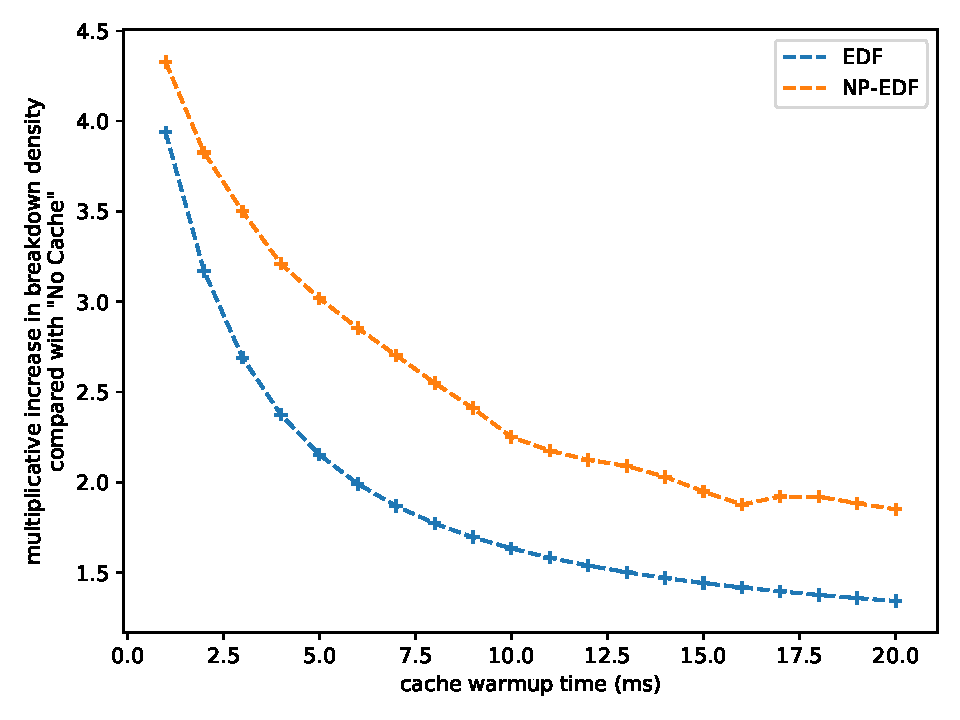
\includegraphics[width=10cm]{uniprocessor_breakdown_density_vs_cache_warmup.pdf}
	\caption{Improvement in breakdown density by adding an L3 cache under EDF and NP-EDF scheduling as $t_\text{warmup}$ varies.}
	\label{fig:uniprocessor_cache_warmup_plots}
\end{figure}

This has interesting consequences on systems in which non-preemptive tasks coexist with preemptive ones, such as those including shared resources and lengthy non-preemptive critical sections. In these cases, increasing the cache performance of a real-time system may improve the schedulability of non-preemptive tasks relative to the schedulability of the system as a whole.

\subsection{Effect of Cache on Multiprocessor Breakdown Density}

We repeat the experiment from \secref{sec:uniprocessor_breakdown_density_experiments} and evaluate the breakdown densities when scheduling on a system with four processors, each with an independent set of caches. The resulting breakdown densities are shown in \tabref{table:multiprocessor_L1_L2_L3_experiment}.

\begin{table}
	\centering
	\resizebox{\textwidth}{!}{%
	\begin{tabular}{|c|c|c|c|c||c|c|c|c|}
		\hline Scheme & G-EDF & G-LLF & G-RM & G-DM & G-NP-EDF & G-NP-LLF & G-NP-RM & G-NP-DM\\\hline
		No cache&4.8609&4.7003&4.6702&4.6210&3.3274&3.3094&3.2952&3.3055\\
		L3 cache&10.9861&8.4322&10.1298&10.1382&7.7722&7.6358&7.6753&7.7449\\
		L2 cache&70.0849&31.3454&66.8809&66.3103&48.5926&41.7282&47.8446&48.1486\\
		L1 cache&241.8332&93.1622&231.8590&229.6940&168.1699&144.5819&165.5736&166.6809\\\hline
	\end{tabular}
	}
	
	\phantom{spacing}
	
	\resizebox{\textwidth}{!}{%
	\begin{tabular}{|c|c|c|c|c||c|c|c|c|}
		\hline Scheme & GR-EDF & GR-LLF & GR-RM & GR-DM & GR-NP-EDF & GR-NP-LLF & GR-NP-RM & GR-NP-DM\\\hline
		No cache&4.3334&4.1036&4.0767&4.0461&3.3274&3.3094&3.2952&3.3055\\
		L3 cache&10.0086&7.2250&9.3830&9.3476&7.7722&7.6358&7.6753&7.7449\\
		L2 cache&62.4484&30.01839&57.7688&57.5439&48.5926&41.7282&47.8446&48.1486\\
		L1 cache&214.5516&92.8252&201.7070&200.5224&168.1699&144.5819&165.5736&166.6809\\\hline
	\end{tabular}
	}

	\caption{Average breakdown densities from our multiprocessor experiment under the four overhead schemes representing effective use of the various caches in the typical memory hierarchy. A prefix of ``GR-'' denotes a global scheduling algorithm where migration is restricted such that tasks may only migrate between jobs.}
	\label{table:multiprocessor_L1_L2_L3_experiment}
\end{table}

As with the uniprocessor case, LLF scheduling is the worst performing of the global schemes considered here due to its excessive context switching. 

Note that the non-preemptive policies implicitly have restricted migration since jobs may not be scheduled in parallel with themselves (they must execute sequentially), so there is no difference between the scheduling capabilities of G-NP-EDF and GR-NP-EDF, for example.

On the task set distribution considered here, we see that the global scheduling algorithms perform better than their restricted-migration counterparts, followed by the non-preemptive policies which have the lowest breakdown densities.

However, it's important to note that our overhead model has no extra penalty for jobs that migrate between processors, so these results may not apply in practice. In fact, the average breakdown density of GR-EDF would clearly surpass that of G-EDF if we were to add a particularly large migration overhead here. This is demonstrated in \figref{fig:multiprocessor_preemption_experiment} where we plot the breakdown utilization of the three EDF scheduling policies as the preemption cost $p$ varies in the ``L3 cache'' overhead scheme.

\begin{figure}
	\centering
	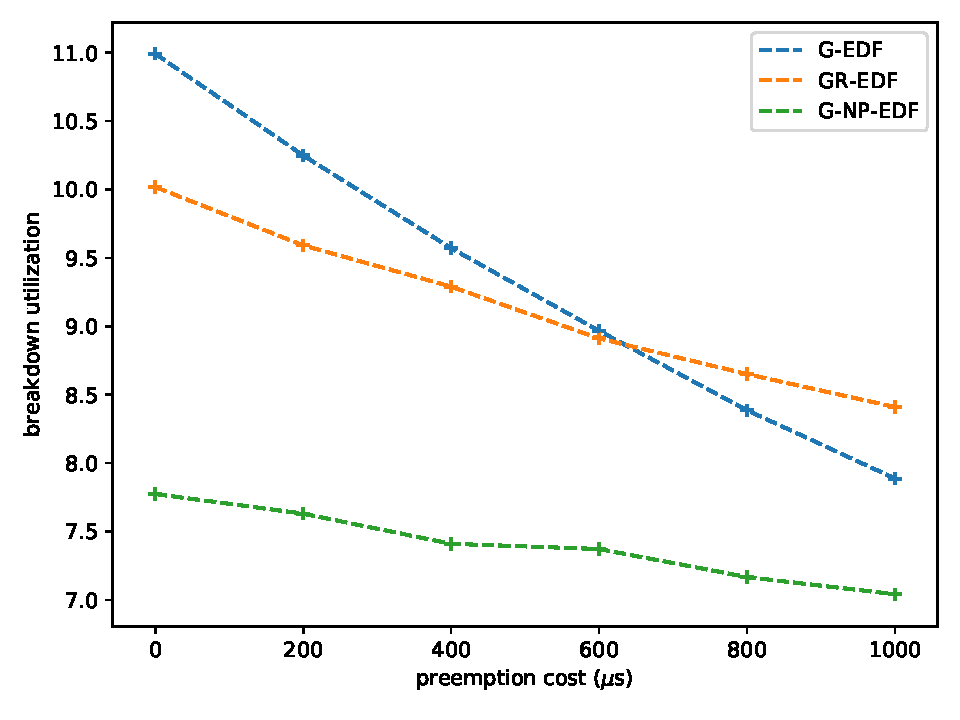
\includegraphics[width=10cm]{multiprocessor_preemption.pdf}
	\caption{Breakdown densities under G-EDF, GR-EDF, and G-NP-EDF as the preemption cost $p$ varies in the ``L3 cache'' overhead scheme.}
	\label{fig:multiprocessor_preemption_experiment}
\end{figure}

Note that when preemption costs are completely removed, GR-EDF achieves a breakdown density of ${\sim}10$. Even under our cache scheme with the largest warmup time (and thus, the greatest indirect preemption penalty), G-EDF's breakdown density does not fall to this level until the preemption cost reaches $p\approx 300$ $\mu$s, which is unreasonable under our model where $p$ only accounts for direct context-switching costs. Hence, for realistic overhead parameters and without a more complicated cache model, we do not expect that GR-EDF would exceed the scheduling performance of G-EDF on the task systems considered here.

As in \secref{sec:uniprocessor_breakdown_density_experiments}, we also analyze the relative effects of cache on the restricted-migration and non-preemptive workloads. To this end, we plot the average breakdown densities in the ``L3 cache'' overhead scheme as $t_\text{warmup}$ varies in \figref{fig:multiprocessor_cache_warmup_plots}.

\begin{figure}
	\centering
	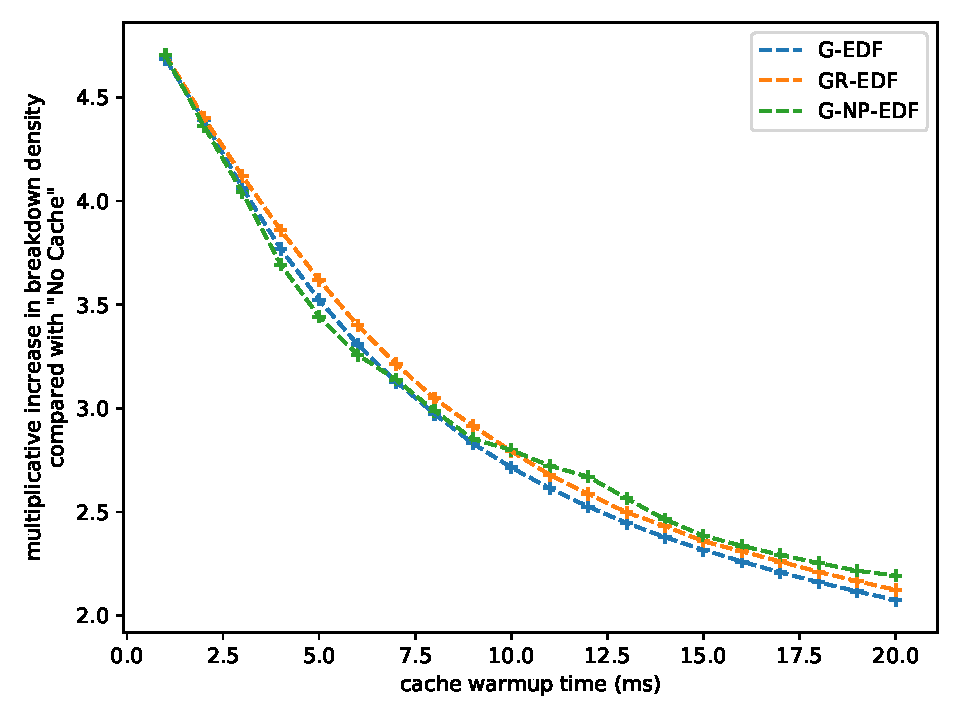
\includegraphics[width=10cm]{multiprocessor_breakdown_density_vs_cache_warmup.pdf}
	\caption{Improvement in breakdown density by adding an L3 cache under G-EDF, GR-EDF, and G-NP-EDF scheduling as $t_\text{warmup}$ varies.}
	\label{fig:multiprocessor_cache_warmup_plots}
\end{figure}

Here, the addition of a cache improves the schedulability of GR-EDF more than G-EDF, but the effect is much less pronounced than in the uniprocessor case. For the caches with large warmup time, GR-NP-EDF sees the most benefit (since its jobs are never preempted), followed by GR-EDF (where the migration restriction makes preemptions less common), and finally G-EDF.

However, the improvement of one scheme over another is very minor and as the warmup time decreases, G-EDF and GR-EDF behave in effectively the same way (in fact, some of the differences are likely due to scheduling anomalies). Thus, on this particular distribution of task systems, relative scheduling performance appears to be affected by the algorithm of choice moreso than any cache effects.

\section{Conclusions and Future Work}
\label{sec:Conclusion}

We have presented a simulation environment for real-time scheduling that implements several uniprocessor and multiprocessor scheduling algorithms while accounting for common overheads by directly simulating context switches and cache behavior. We have also shown that it can be effectively used to construct simulation studies to help analyze the performance of task systems under various cache setups. Such studies would be valuable when porting a real-time system to new architectures with different memory hierarchies.

Moreover, we expect that our tool could be used as a teaching aid as it can rapidly construct schedules for example task systems and would allow for a visual comparison of how various scheduling policies differ.

Future work could focus on adding more complicated scheduling algorithms to the simulator and expanding the overhead model to account for migration penalties. Further work could model caches that are shared between processors and more accurately simulate cache eviction such that jobs may maintain some cached data after preemption.

In \secref{sec:uniprocessor_breakdown_density_experiments}, we noted that caches necessarily affect non-preemptive workloads more heavily than preemptive ones. As such, one could investigate the behavior of scheduling algorithms on task systems in which some jobs must run without interruption (e.g.\ those involving shared resource control).

\bibliographystyle{plain}
\begin{thebibliography}{99}%\setlength{\itemsep}{-1ex}
	% \small
	\singlespace
	
	\bibitem{Baruah} Baruah, Sanjoy K., et al. ``Feasibility Problems for Recurring Tasks on One Processor.'' {\em Selected Papers of the 15th International Symposium on Mathematical Foundations of Computer Science, Elsevier Science Publishers B. V.}, 1993, pp. 3–20. ACM Digital Library, http://dl.acm.org/citation.cfm?id=162625.162629.
	
	\bibitem{Cerqueira} Cerqueira, Felipe, and Björn B. Brandenburg. A Comparison of Scheduling Latency in Linux, PREEMPT-RT, and LITMUS RT. 2013.
		
	\bibitem{Diaz} Diaz, Arnoldo, et al. ``Realtss: A Real-Time Scheduling Simulator.'' {\em 2007 4th International Conference on Electrical and Electronics Engineering}, 2007, pp. 165–68. IEEE Xplore, doi:10.1109/ICEEE.2007.4344998.
	
	\bibitem{Leung} Leung, Joseph Y. T., and M. L. Merrill. ``A Note on Preemptive Scheduling of Periodic, Real-Time Tasks.'' {\em Information Processing Letters, vol. 11, no. 3}, Nov. 1980, pp. 115–18. ScienceDirect, doi:10.1016/0020-0190(80)90123-4.
	
	\bibitem{Intel} Intel 64 and IA-32 Architectures Software Developer’s Manual, Volume 1: Basic Architecture. p. 502.	
	
	\bibitem{Levinthal} Levinthal, Dr David. Performance Analysis Guide for Intel® Core™ I7 Processor and Intel® Xeon™ 5500 Processors. p. 72.

	\bibitem{Li} Li, Chuanpeng, et al. ``Quantifying the Cost of Context Switch.'' Proceedings of the 2007 Workshop on Experimental Computer Science, ACM, 2007. ACM Digital Library, doi:10.1145/1281700.1281702.
	
	\bibitem{Manacero} Manacero, A., et al. ``Teaching Real-Time with a Scheduler Simulator.'' {\em 31st Annual Frontiers in Education Conference. Impact on Engineering and Science Education. Conference Proceedings (Cat. No.01CH37193)}, vol. 2, 2001, pp. T4D-15. IEEE Xplore, doi:10.1109/FIE.2001.963651.
	
	\bibitem{McVoy} McVoy, Larry, and Carl Staelin. ``Lmbench: Portable Tools for Performance Analysis.'' Proceedings of the 1996 Annual Conference on USENIX Annual Technical Conference, USENIX Association, 1996, pp. 23–23. ACM Digital Library, http://dl.acm.org/citation.cfm?id=1268299.1268322.
	
	\bibitem{Singhoff} Singhoff, F., et al. ``Cheddar: A Flexible Real Time Scheduling Framework.'' {\em Proceedings of the 2004 Annual ACM SIGAda International Conference on Ada: The Engineering of Correct and Reliable Software for Real-Time \& Distributed Systems Using Ada and Related Technologies}, ACM, 2004, pp. 1–8. ACM Digital Library, doi:10.1145/1032297.1032298.
	
	\bibitem{Srinivasan} Srinivasan, Anand, and James H. Anderson. ``Optimal Rate-Based Scheduling on Multiprocessors.'' {\em Journal of Computer and System Sciences}, vol. 72, no. 6, Sept. 2006, pp. 1094–117. ScienceDirect, doi:10.1016/j.jcss.2006.03.001.
\end{thebibliography}
\end{document}